\subsection{例：質量ばねダンパを古典制御で設計する}

質量 $m$、粘性 $c$、ばね $k$ の対象に力 $u$ を加える。
\begin{equation}
  m\ddot{q}+c\dot{q}+kq=u
\end{equation}
初期値 0 でラプラス変換すると
\begin{align}
  m s^2Q(s)+csQ(s)+kQ(s)&=U(s),\\
  (ms^2+cs+k)Q(s)&=U(s),\\
  G(s)=\frac{Q(s)}{U(s)}&=\frac{1}{ms^2+cs+k}.
\end{align}
標準形と比べるために分母を $m$ で割る。
\begin{equation}
  G(s)=\frac{1/m}{s^2+(c/m)s+k/m}.
\end{equation}
二次標準形 $s^2+2\zeta\omega_ns+\omega_n^2$ と係数を比べると
\begin{align}
  \omega_n^2&=k/m,\\
  2\zeta\omega_n&=c/m.
\end{align}
よって
\begin{align}
  \omega_n&=\sqrt{k/m},\\
  \zeta&=\frac{c}{2\sqrt{mk}}.
\end{align}
このように、物理パラメータ $m,c,k$ は応答仕様 $\omega_n,\zeta$ に直接つながる。重い質量は遅くし、大きな粘性は減衰を増やし、大きなばねは固有周波数を上げる。

比例制御 $u=K_p(r-q)$ を入れると
\begin{equation}
  m\ddot{q}+c\dot{q}+kq=K_p(r-q)
\end{equation}
である。整理して
\begin{equation}
  m\ddot{q}+c\dot{q}+(k+K_p)q=K_pr
\end{equation}
となる。閉ループの固有角周波数は
\begin{equation}
  \omega_{n,cl}=\sqrt{\frac{k+K_p}{m}}
\end{equation}
であり、減衰比は
\begin{equation}
  \zeta_{cl}=\frac{c}{2\sqrt{m(k+K_p)}}.
\end{equation}
したがって $K_p$ を大きくすると速くなるが、粘性 $c$ が変わらなければ減衰比は下がり、振動しやすくなる。これは「ゲインを上げると速いが振動する」という経験則の式による説明である。

比例制御の振動を抑えたいときは、変位の測定値から速度 $\dot{q}$ も使う。目標値をステップ状に変える例では、微分キックを避けるために微分を偏差ではなく測定値へかけ、
\begin{equation}
  u=K_p(r-q)-K_d\dot{q}
\end{equation}
とする。この PD 制御を代入すると
\begin{equation}
  m\ddot{q}+(c+K_d)\dot{q}+(k+K_p)q=K_pr
\end{equation}
である。閉ループの固有角周波数は比例制御と同じ
\begin{equation}
  \omega_{n,cl}=\sqrt{\frac{k+K_p}{m}}
\end{equation}
だが、減衰比は
\begin{equation}
  \zeta_{cl}=
  \frac{c+K_d}{2\sqrt{m(k+K_p)}}
\end{equation}
に変わる。したがって $K_d$ は、速さを大きく変えずに振動を抑える減衰として働く。ただし定常状態では $\dot{q}=0$ なので、PD 制御だけでは比例制御と同じ静的なばね負荷を残す。ステップ目標値 $r$ に対する定常値は
\begin{equation}
  q_\infty=\frac{K_p}{k+K_p}r
\end{equation}
であり、$k>0$ なら $q_\infty\neq r$ である。

定常偏差も消したい場合は、積分状態 $\eta$ を加えて
\begin{align}
  u&=K_p(r-q)+\eta-K_d\dot{q},\\
  \dot{\eta}&=K_I(r-q)
\end{align}
とする。一定目標値で閉ループが安定なら、定常状態では $\dot{\eta}=0$ だから $r-q=0$、すなわち $q=r$ である。このとき積分状態は、ばねをつり合わせるための力 $\eta=kr$ を供給する。偏差を消せる一方で、積分器は閉ループへ状態を一つ増やす。$r$ を一定として平衡点まわりの偏差を考えると、PID 候補の特性多項式は
\begin{equation}
  ms^3+(c+K_d)s^2+(k+K_p)s+K_I
\end{equation}
になる。三次の Routh-Hurwitz 判別法から、係数が正で
\begin{equation}
  (c+K_d)(k+K_p)>mK_I
\end{equation}
を満たすことが安定の基本条件になる。積分ゲイン $K_I$ を大きくすれば偏差の戻りは速くなるが、この条件と入力の大きさを同時に確認する必要がある。

\wfig{mass-spring-design-examples} は、同じ対象
\begin{equation}
  m=1\,\mathrm{kg},\qquad
  c=1\,\mathrm{N\,s/m},\qquad
  k=1\,\mathrm{N/m}
\end{equation}
に、$r=1\,\mathrm{m}$ のステップ目標値を与えた比較である。三つの候補は
\begin{equation}
  \begin{array}{c|ccc}
  \text{候補} & K_p & K_d & K_I\\ \hline
  \text{P} & 5 & 0 & 0\\
  \text{PD} & 5 & 3 & 0\\
  \text{PID} & 5 & 3 & 2
  \end{array}
\end{equation}
である。P 制御は初期の力が大きく、速く動くが、ばねを押し切る定常力が不足するため残留偏差を持つ。PD 制御は $K_d$ によって振動を抑えるが、低周波のゲインは P 制御と同じなので定常偏差は残る。PID 制御は積分状態がばね力を補うため目標値へ近づくが、操作力を長く使う。設計では、応答の速さだけでなく、終端偏差、最大力、RMS 操作力のような入力側の指標も同時に評価する。

\begin{figure}[tbp]
\centering
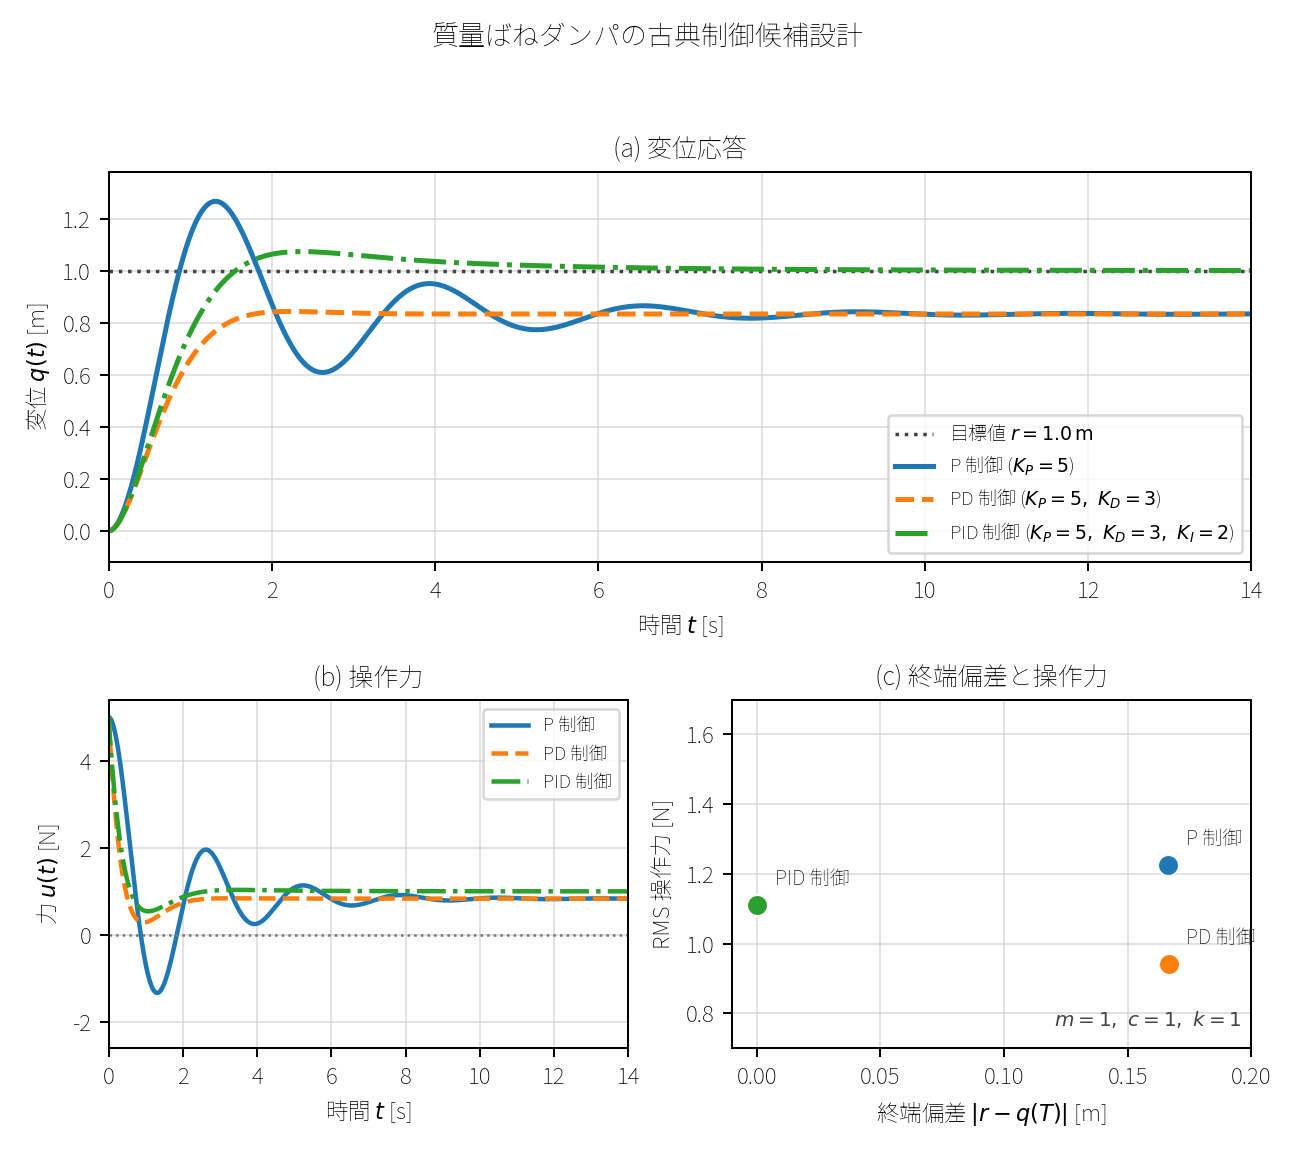
\includegraphics[width=0.96\linewidth,bb=0 0 1296 1152]{figures/mass_spring_design_examples.png}
\caption{質量ばねダンパ系に対する P、PD、PID 候補設計の比較。対象は $m=1\,\mathrm{kg}$、$c=1\,\mathrm{N\,s/m}$、$k=1\,\mathrm{N/m}$、目標値は $r=1\,\mathrm{m}$ である。PD 制御は速度フィードバックで振動を抑え、PID 制御は積分状態で定常偏差を減らすが、操作力の使い方も変わる。}
\label{fig:mass-spring-design-examples}
\end{figure}

\wfig{mass-spring-design-examples} の数値は、上の式だけでも読み取れる。P 制御と PD 制御では積分器がないので、一定目標値に対する定常力の釣合いは
\begin{equation}
  kq_\infty=K_p(r-q_\infty),\qquad
  q_\infty=\frac{K_p}{k+K_p}r=\frac{5}{6}\,\mathrm{m}
\end{equation}
である。したがって、どちらも目標値 $1\,\mathrm{m}$ に対して約 $0.167\,\mathrm{m}$ の残留偏差を持つ。PD 制御が改善しているのは定常値ではなく、二次閉ループの減衰である。固有角周波数は $\omega_n=\sqrt{(k+K_p)/m}=\sqrt{6}\,\mathrm{rad/s}$、減衰比は
\begin{equation}
  \zeta=\frac{c+K_d}{2\sqrt{m(k+K_p)}}
\end{equation}
だから、P 制御では $\zeta=1/(2\sqrt{6})\simeq0.204$、PD 制御では $\zeta=4/(2\sqrt{6})\simeq0.816$ になる。この増加が、上段の振動とオーバーシュートの小ささに対応している。

PID 候補では、積分ゲインを入れても Routh-Hurwitz 条件を満たす必要がある。ここでは
\begin{equation}
  (c+K_d)(k+K_p)=4\cdot6=24>mK_I=2
\end{equation}
であり、少なくとも三次線形モデルの安定条件は満たしている。図の下段右では、この安定な PID 候補が終端偏差をほぼ $0\,\mathrm{m}$ まで減らす一方、RMS 操作力は PD 制御の約 $0.94\,\mathrm{N}$ より大きい約 $1.11\,\mathrm{N}$ になっている。三候補はいずれも初期操作力が $u(0)=K_pr=5\,\mathrm{N}$ で、ピーク力だけでは差が出ない。このため、同じピーク力の範囲でも、PD 制御は平均的な入力を抑えて振動を減らし、PID 制御は残留偏差を消す代わりに操作力を長く使う、という入力側のトレードオフが残る。
